\fancyhead[LE]{\fontsize{8.5pt}{10pt}\selectfont\textbf{\textsf{\thepage}}\quad \textbf{\textsf{CHƯƠNG 1}}\quad \textsf{Các hàm số và Mô hình}}
\fancyhead[RO]{\fontsize{8.5pt}{10pt}\selectfont\textsf{MỤC 1.1}\quad \textbf{\textsf{\thepage}}}

\setcounter{page}{50}

\noindent
\begin{minipage}[t]{0.265\textwidth}
    \fontsize{8pt}{10.5pt}\selectfont
    \vspace*{46pt}
    \begin{center}
        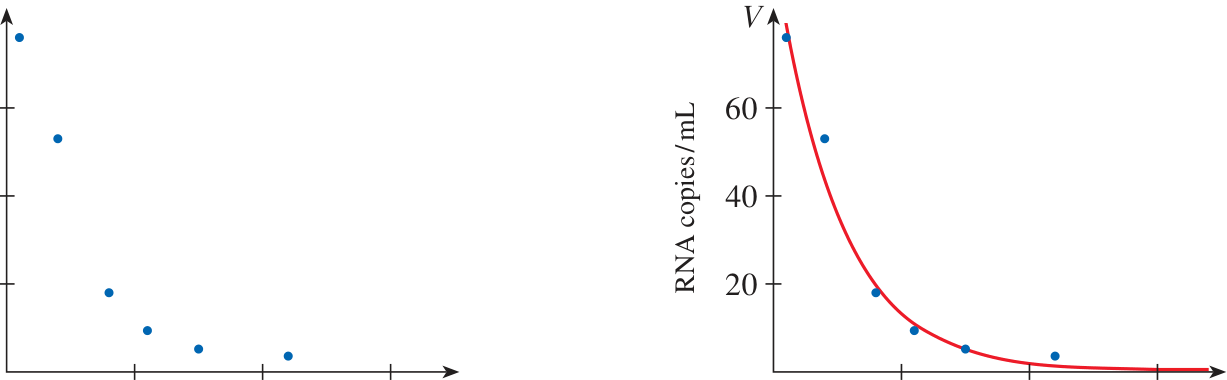
\includegraphics[width=0.92\linewidth]{images/p0085_fig10.png}
        
        \vspace{3pt}
        {\raggedright\textbf{\textsf{HÌNH 10}}\\
        Tải lượng virus trong huyết tương ở bệnh nhân 303\par}
    \end{center}
    
    \vspace{210pt}
    \begin{center}
        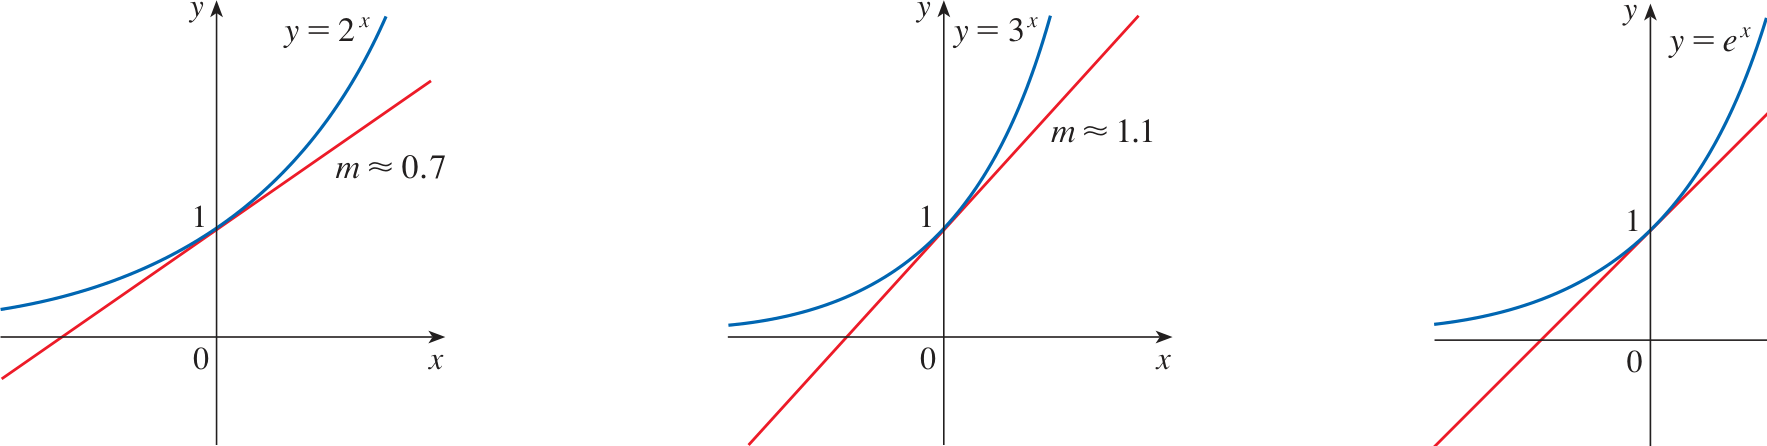
\includegraphics[width=0.92\linewidth]{images/p0085_fig12.png}
        
        \vspace{3pt}
        {\raggedright\textbf{\textsf{HÌNH 12}}\par}
    \end{center}
\end{minipage}%
\hfill
\begin{minipage}[t]{0.708\textwidth}
    \fontsize{9.3pt}{13.4pt}\selectfont
    dạng hàm $y = a \cdot b^t$, ta nhận được mô hình
    \[ V = 96{,}39785 \cdot (0{,}818656)^t \]
    Ở Hình 11, ta vẽ đồ thị hàm số mũ này cùng với các điểm dữ liệu và nhận thấy rằng mô hình biểu diễn tải lượng virus khá tốt trong tháng điều trị đầu tiên.

    \vspace{0.6em}
    \begin{center}
        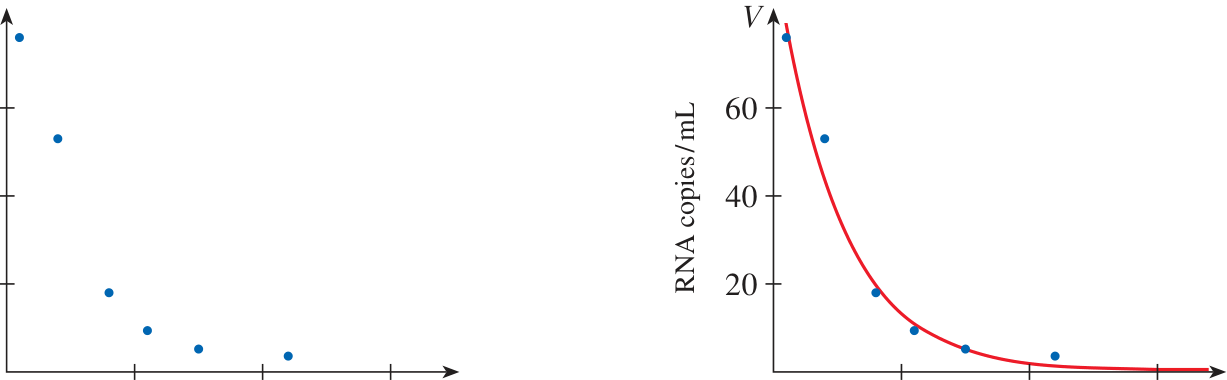
\includegraphics[width=0.72\linewidth]{images/p0085_fig11.png}
        
        \vspace{2pt}
        {\raggedright\textbf{\textsf{HÌNH 11}}\\
        Mô hình hàm mũ cho tải lượng virus \hfill{\color{stewartcyan}$\blacksquare$}\par}
    \end{center}
    \vspace{0.8em}

    Trong Ví dụ 3, chúng ta đã sử dụng hàm số mũ có dạng $y = a \cdot b^t, b > 1$, để mô hình hóa sự tăng trưởng dân số và trong Ví dụ 4, chúng ta đã dùng $y = a \cdot b^t, b < 1$, để mô hình hóa sự suy giảm tải lượng virus. Trong Mục 3.8, chúng ta sẽ tìm hiểu thêm các ví dụ về các đại lượng tăng trưởng hoặc suy giảm theo hàm mũ, bao gồm giá trị của một tài khoản đầu tư sinh lãi kép và lượng chất phóng xạ còn lại khi vật chất phân rã.

    \vspace{1.2em}
    \noindent{\color{stewartcyan}\rule{1.1ex}{1.1ex}}\hspace{0.5em}{\large\textbf{\textsf{Số }}} $\boldsymbol{e}$
    \vspace{0.5em}

    Trong tất cả các cơ số khả dĩ của một hàm số mũ, có một cơ số thuận tiện nhất cho các mục đích của giải tích. Việc lựa chọn cơ số $b$ chịu ảnh hưởng bởi cách mà đồ thị $y = b^x$ cắt trục $y$. Các Hình 12 và 13 cho thấy các tiếp tuyến với đồ thị của $y = 2^x$ và $y = 3^x$ tại điểm $(0, 1)$. (Tiếp tuyến sẽ được định nghĩa chính xác trong Mục 2.7. Đối với mục đích hiện tại, bạn có thể hình dung tiếp tuyến của đồ thị hàm mũ tại một điểm là đường thẳng chỉ chạm vào đồ thị tại duy nhất điểm đó.) Nếu ta đo hệ số góc của các tiếp tuyến này tại $(0, 1)$, ta thấy rằng $m \approx 0{,}7$ đối với $y = 2^x$ và $m \approx 1{,}1$ đối với $y = 3^x$.

    Hóa ra, như chúng ta sẽ thấy trong Chương 3, một số công thức của giải tích sẽ được đơn giản hóa đáng kể nếu ta chọn cơ số $b$ sao cho hệ số góc của tiếp tuyến với $y = b^x$ tại $(0, 1)$ bằng \emph{chính xác} 1. (Xem Hình 14.) Trên thực tế, \emph{có} một số như vậy và nó được ký hiệu bởi chữ cái $e$. (Ký hiệu này được nhà toán học Thụy Sĩ Leonhard Euler lựa chọn vào năm 1727, có lẽ vì đó là chữ cái đầu tiên của từ \emph{exponential} - hàm mũ.) Xét theo

    \vspace{1.2em}
    \begin{center}
        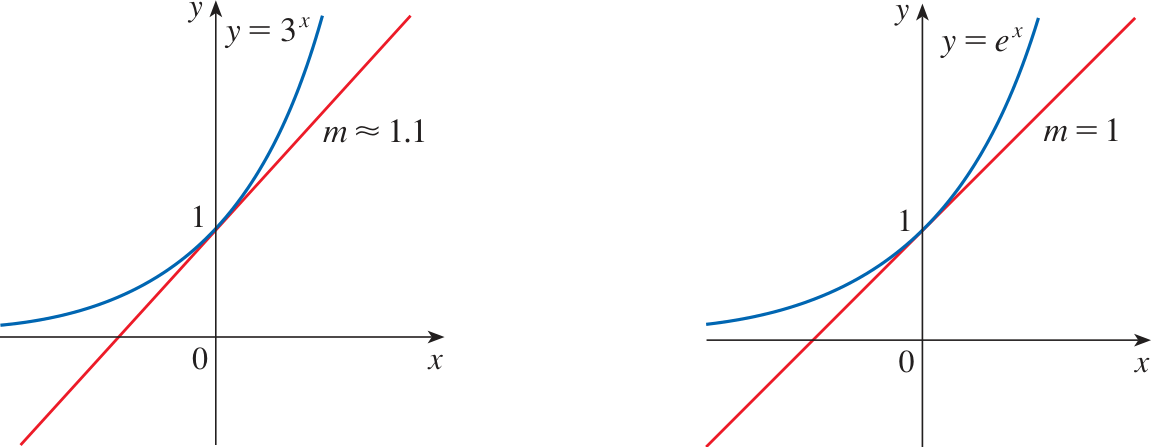
\includegraphics[width=0.92\linewidth]{images/p0085_fig14.png}
        
        \vspace{2pt}
        \parbox{0.48\linewidth}{\centering\textbf{\textsf{HÌNH 13}}}\hfill
        \parbox{0.48\linewidth}{\centering\textbf{\textsf{HÌNH 14}}}
    \end{center}
\end{minipage}